\subsection{Brute force geometric comparison}

%
% How does the algorithm work. Robustness
%
Our default brute force approach implementation runs per triangle pair through all possible geometric
configurations (Algorithm \ref{algorithm:bf}).
Firstly, we determine the distances between each line-segment to line-segment combination (segment-to-segment stage).
Second, with all six involved vertices we compute the distance to the other triangle (point-to-triangle stage).
This yields fifteen comparisons in total. The distance between two triangles is the minimum over all computed distances.
The brute force method is a robust approach, it always yields the correct answer after the evaluation of all steps. A fusion of multiple steps is not possible because all configurations have to be evaluated naively as seen in Appendix:Algorithms \ref{algorithm:point_to_triangle}, \ref{algorithm:seg_seg}.

The calculation of distance between line segments \cite{Ericson2005} in 3D involves extending the line segments until intersection, then the closest point on the two segments is on the boundaries.
The segment $S1 = [P0, P1]$ can be formulated as $P(s) = P0+s(P1-P0) = P0+su$ with a constraint, $0<=s<=1$. Similarly, $S2 = [Q0, Q1]$
is written as $Q(t) = Q0+t(Q1-Q0) = Q0+tu$ with constraint $0<=t<=1$. So, for $sC$ and $tC$ being the closest points on the corresponding extended segments lines L1 and L2, then if  both sC and tC are within the boundaries of the segments then the closest points are also the closest points on the respective segments. 
In the case where sC and tC correspond to points on L1 and L2 outside the range of either segment $S1$ and $S2$, then sC and tC do not also define the closest points on the segments $S1$ and $S2$. So it is necessary to determine points that minimize 
$w(s,t) = P(s) - Q(t)$ over the ranges of the segments using the corresponding constraints. 
The problem can be formulated into a minimization problem where the equation w is the same as minimizing 
$|w|^2 = w \cdot w= (P0+su-tv) \cdot (Q0+su-tv)$. The relation of $|w|^2$ define a equation over a (s,t)-plane (See figure \ref{figure:ss_regions}) with a minimum at $C = (sC, tC)$, it is strictly growing along the (s,t)-plane with starting point from C. The required minimum region is not C but it is located over a subregion G of the (s,t)-plane. Using this method it is possible to perform checks to find the minimum of w(s,t) that correspond to the minimum distance between the segments.

\begin{figure}[!h]
\centering

\includegraphics[width=0.3\textwidth]{sketches/ss_box} 
\caption{(s,t) parameter space with G boundary box C for global minimum}
\label{figure:ss_regions}
\end{figure} 

The next stage of the brute force algorithm requires checking the point-to-triangle distance \ref{Eberly1999}. Using triangle T barymetic function such that $T(s, t) = B + s \cdot BA + t \cdot DA$ where $B = A$, $BA = B - A$, $DA = D - A$ for $(s,t) \in D = \{(s,t) : s \in [0,1],t \in [0,1],s + t ≤ 1\}$. The minimum distance is computed by the values $(s, t) \in D$ in distance equation $Q(s, t) = |T(s, t) - P|^2$ where $T(s,t)$ correspond to a point Q. The function can be written as: 
$Q(s,t)=as^2 +2bst+ct^2 +2ds+2et+f$ where $a = BA \cdot BA$, $b = BA \cdot DA$, $c = D-A \cdot DA$, $d = B-A \cdot (B - P)$, $e = DA \cdot (B - P)$, and $f = (B - P) \cdot (B - P)$. So for function Q, $ac - b2$ = $(B-A \cdot B-A)(E1 \cdot D) - (B-A \cdot B-A)^2$ =$|B-A \cdot D-A|^2 >0$. The positivity is based on the assumption that the two edges $B-A$, $D-A$ are linearly independent. The minimum occurs at an interior point of D where the gradient $\nabla Q = 2(as + bt + d, bs + ct + e) = (0, 0)$ or at a point on the boundary of D. The gradient of Q is zero only when $s = (be - cd)/(ac - b^2)$ and $t = (bd - ae)/(ac - b^2).$  If $(s,t) \in D$ (See Figure \ref{figure:pt_regions}) then minimum of Q is found. 

\begin{figure}[!h]
\centering
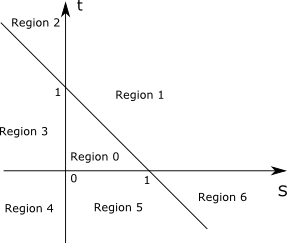
\includegraphics[width=0.4\textwidth]{sketches/pt_regions} 
\caption{Regions based on the (s,t) parameters plane}
\label{figure:pt_regions}
\end{figure}

On the other hand if the minimum is not in D then it is on the boundary of the triangle. Using the active constraints we restrict the solution so if (s, t) is in region one then the level curves of Q are constant. As the level value V increase from $V_{min}$ as they growing away from $(s,t)$ there is a smallest level value that is tangent to the  domain $D$ with $s+t = 1$. So for any level values $V < V_{min}$, the corresponding do not intersect $D$. However for any portion of $D$ that intersect levels V must be $V > V_{min}$. Therefore in this case point $(s0, t0)$ provides the minimum distance between P and the triangle where $t0$ is known $t0 = 1 - s0$ and $s0$ is the only unknown to be solved. Moreover, when minimization is happening at $\nabla Q(s, 1 − s) = 0$ then there are three cases where $s > 1$ and $s$ has to be restricted to $s=1$ and the minimum occurs at $\nabla Q(1, 0)$ because of the constraints. Similarly if $s < 0$ then minimum occurs when $\nabla Q(0,1)$ or lastly $s \in [0,1]$. Similarly the same technique for determining whether the minimum occurs at the endpoints or at the interior interval of the corresponding constraints is performed for all regions.

